%%%%%%%%%%%%%%%%%%%%%%%%%%%%%%%%%%%%%%%%%
% Beamer Presentation
% LaTeX Template
% Version 1.0 (10/11/12)
%
% This template has been downloaded from:
% http://www.LaTeXTemplates.com
%
% License:
% CC BY-NC-SA 3.0 (http://creativecommons.org/licenses/by-nc-sa/3.0/)
%
%%%%%%%%%%%%%%%%%%%%%%%%%%%%%%%%%%%%%%%%%

%----------------------------------------------------------------------------------------
%	PACKAGES AND THEMES
%----------------------------------------------------------------------------------------

\documentclass{beamer}


\mode<presentation> {

% The Beamer class comes with a number of default slide themes
% which change the colors and layouts of slides. Below this is a list
% of all the themes, uncomment each in turn to see what they look like.

%\usetheme{default}
%\usetheme{AnnArbor}
%\usetheme{Antibes}
%\usetheme{Bergen}
%\usetheme{Berkeley}
%\usetheme{Berlin}
%\usetheme{Boadilla}
%\usetheme{CambridgeUS}
%\usetheme{Copenhagen}
%\usetheme{Darmstadt}
%\usetheme{Dresden}
%\usetheme{Frankfurt}
%\usetheme{Goettingen}
%\usetheme{Hannover}
%\usetheme{Ilmenau}
%\usetheme{JuanLesPins}
%\usetheme{Luebeck}
\usetheme{Madrid}
%\usetheme{Malmoe}
%\usetheme{Marburg}
%\usetheme{Montpellier}
%\usetheme{PaloAlto}
%\usetheme{Pittsburgh}
%\usetheme{Rochester}
%\usetheme{Singapore}
%\usetheme{Szeged}
%\usetheme{Warsaw}

% As well as themes, the Beamer class has a number of color themes
% for any slide theme. Uncomment each of these in turn to see how it
% changes the colors of your current slide theme.

%\usecolortheme{albatross}
%\usecolortheme{beaver}
%\usecolortheme{beetle}
%\usecolortheme{crane}
%\usecolortheme{dolphin}
%\usecolortheme{dove}
%\usecolortheme{fly}
%\usecolortheme{lily}
%\usecolortheme{orchid}
%\usecolortheme{rose}
%\usecolortheme{seagull}
%\usecolortheme{seahorse}
%\usecolortheme{whale}
%\usecolortheme{wolverine}

%\setbeamertemplate{footline} % To remove the footer line in all slides uncomment this line
%\setbeamertemplate{footline}[page number] % To replace the footer line in all slides with a simple slide count uncomment this line

%\setbeamertemplate{navigation symbols}{} % To remove the navigation symbols from the bottom of all slides uncomment this line
}

\usepackage{macros}

%----------------------------------------------------------------------------------------
%	TITLE PAGE
%----------------------------------------------------------------------------------------

\title[Short title]{Bandit Problem and UCB} % The short title appears at the bottom of every slide, the full title is only on the title page

\author{Subhojyoti Mukherjee} % Your name
\institute[IIT Madras] % Your institution as it will appear on the bottom of every slide, may be shorthand to save space
{
IIT Madras \\ % Your institution for the title page
\medskip
%\textit{john@smith.com} % Your email address
}
\date{\today} % Date, can be changed to a custom date

\begin{document}
\nocite{*}
\begin{frame}
\titlepage % Print the title page as the first slide
\end{frame}

\begin{frame}
\frametitle{Overview} % Table of contents slide, comment this block out to remove it
\tableofcontents % Throughout your presentation, if you choose to use \section{} and \subsection{} commands, these will automatically be printed on this slide as an overview of your presentation
\end{frame}

%----------------------------------------------------------------------------------------
%	PRESENTATION SLIDES
%----------------------------------------------------------------------------------------


\section{Introduction}
\begin{frame}
\frametitle{Introduction}
\begin{itemize}
\item<1-> The bandit problem is a sequential decision making process where at each timestep we have to choose one action or arm from a set of arms. 
\item<2-> After say pulling each arm once we are presented with an \emph{exploration-exploitation}  problem, that is whether to continue to pull the arm for which we have observed the highest estimated reward till now(exploitation) or to explore a new arm(exploration). 
\item<3-> If we become too greedy and always exploit we may miss the chance of actually finding the optimal arm and get stuck with a sub-optimal arm.
\end{itemize}
\end{frame}

\begin{frame}
\frametitle{Why study bandits at all?}
\begin{itemize}
\item<1-> We all know of $\epsilon$-greedy algorithm, we can simply stick to it.
\item<2-> But $\epsilon$-greedy only gives us an asymptotic guarantee. There is no guarantee that in a highly regressive environment how $\epsilon$-greedy will behave. Can we be better in our search?
\item<3-> Bandits allows us to study this behavior in a more formal way giving us strict guarantees regarding the performance of our algorithm.
\item<4-> They form the linking pieces of a larger problem.
\item<5-> They are easy to implement.    
\end{itemize}
\end{frame}

\begin{frame}
\frametitle{Some practical applications}
\begin{itemize}
\item<1-> Selecting the best channel (out of several existing channels) for mobile communications in a very short duration.
\item<2-> Selecting a small set of best workers (out of a very large pool of workers) whose productivity is above a threshold.
\item<3-> Selecting the best possible route for a message to pass through in a peer-to-peer network connection.
\end{itemize}
\end{frame}


\section{Stochastic Multi-Armed Bandit Problem}
\begin{frame}
\frametitle{Stochastic Multi-Armed Bandit Problem}
\begin{itemize}
\item<1-> In stochastic multi-armed bandit problem we are presented with a finite set of actions or arms. 
\item<2-> The rewards for each of the arms is drawn from identical and independent distributions. 
\item<3-> The learner does not know the mean of the distributions, denoted by $\mu_{i}$. 
\item<4-> The learner has to find the optimal arm the mean of whose distribution is denoted by $\mu^{*}$ such that $\mu^{*}> \mu_{i}, \forall i\in A$.
\item<5-> The distributions for each of the arms are fixed throughout the time horizon. 
\end{itemize}
\end{frame}

\begin{frame}
\frametitle{Basic Notations}
\begin{itemize}
\item<1-> Goal: To minimize Regret
\item<2->  Average reward of best action is $\mu^{*}$ and any other action $i$ as $\mu_{i}$. There are $K$ total actions. $T_{i}(n)$ is number of times tried action $i$ is executed till $n$-timesteps.
\item<3->  Cumulative Regret: The loss we suffer because of not pulling the optimal arm till the total number of timesteps  $n$. 
\begin{align*}
R_{n}=\mu^{*}n - \sum_{i\in A} \mu_{i}T_{i}(n),
\end{align*}
\item<4->  The expected regret of an algorithm after $n$ rounds can be written as
\begin{align*}
\E[R_{n}]= \sum_{i=1}^K \E[T_{i}(n)] \Delta_i,
\end{align*}
\item<4-> $\Delta_{i}=\mu^{*}-\mu_{i}$ denotes the gap between the means of the optimal arm and of the $i$-th arm. 
\end{itemize}
\end{frame}

\section{UCB1 Algorithm}
\begin{frame}
\frametitle{UCB 1 Algorithm}
\begin{algorithm}[H]
\caption{UCB1}
\begin{algorithmic}[1]
\State Pull each arm once
 \For{$t=K+1,..., T$}
\State Pull the arm such that $\max_{i\in A}\bigg\lbrace\hat{\mu} + \sqrt{\dfrac{2\log t}{n_i}}\bigg\rbrace$
 \EndFor
\end{algorithmic}
\end{algorithm}
\cite{auer2002finite}
\end{frame}

\section{Concentration Bounds}
\begin{frame}
\frametitle{Concentration Bounds}
\begin{itemize}
\item<1-> The issue of coin tossing.
\item<2-> Chernoff-Hoeffding Bounds and its applications.
\item<3-> Let $X_{1}, . . . , X_{n}$ be random variables with common
range [0, 1] and such that $E[X_{t} |X_{1}, . . . , X_{t-1}] = \mu.$ Let $\bar{S_n} = \dfrac{X_{1} +,....,+ X_{n}}{n}$. Then for all $a \geq 0$,
\begin{align*}
\mathbb{P} \lbrace \bar{S_{n}} \geq \mu + a \rbrace \leq e^{-2a^{2}n}\\
\mathbb{P}\lbrace \bar{S}_{n} \leq \mu - a \rbrace \leq e^{-2a^{2}n}
\end{align*}
\end{itemize}
\end{frame}


\section{UCB1 Theorem and Proof}
\begin{frame}
\frametitle{UCB1 Theorem on Regret Bound}
\begin{theorem}
For all $K > 1$, if policy UCB1 is run on K arms having arbitrary reward
distributions $P_{1}, . . . , P_{K}$ with support in $[0, 1]$, then its expected regret after any number $n$ plays is at most,
\begin{align*}
\mathbb{E}[R_n]\leq \sum_{i\in A}\dfrac{8\log n}{\Delta_{i}} + \sum_{i\in A}\Delta_{i}\bigg(1+\dfrac{\pi^{2}}{3}\bigg) 
\end{align*}
where $\mu_{1}, . . . , \mu_{K}$ are the expected values of $P_{1}, . . . , P_{K}$ .
\end{theorem}
\end{frame}

\begin{frame}
\frametitle{UCB1 Proof}
\begin{itemize}
\item<1-> The main goal is to bound the number of pulls ($T_i(n)$) of the sub-optimal arm $i$ till the $n$-th timestep.
\item<2-> So, we will assume that the $i$-th arm has been pulled atleast $\ell$ times and bound the probability of how many times it can be pulled after that.
\begin{align*}
T_{i}(n)&\leq \ell +\sum_{t=K+1}^{n}\lbrace I_t=i, T_i(t-1)\geq \ell\rbrace
\end{align*}
\item<3-> But, this is nothing but the probability that how many times after the $\ell$ pulls the UCB of $*$ is less than the UCB of $i$ which will have the highest UCB among all arms in $A$ to be selected,
\begin{align*}
T_{i}(n)&\leq \ell + \sum_{t=1}^{\infty}\sum_{s=1}^{t-1}\sum_{s_i =\ell}^{t-1}\lbrace \bar{X}_{s}^{*} + c_{t,s} \leq \bar{X}_{i,s_i} + c_{t,s_i} \rbrace
\end{align*}
\end{itemize}
\end{frame}

\begin{frame}
\frametitle{UCB1 Proof}
\begin{itemize}
\item<1-> The main argument lies in this, 
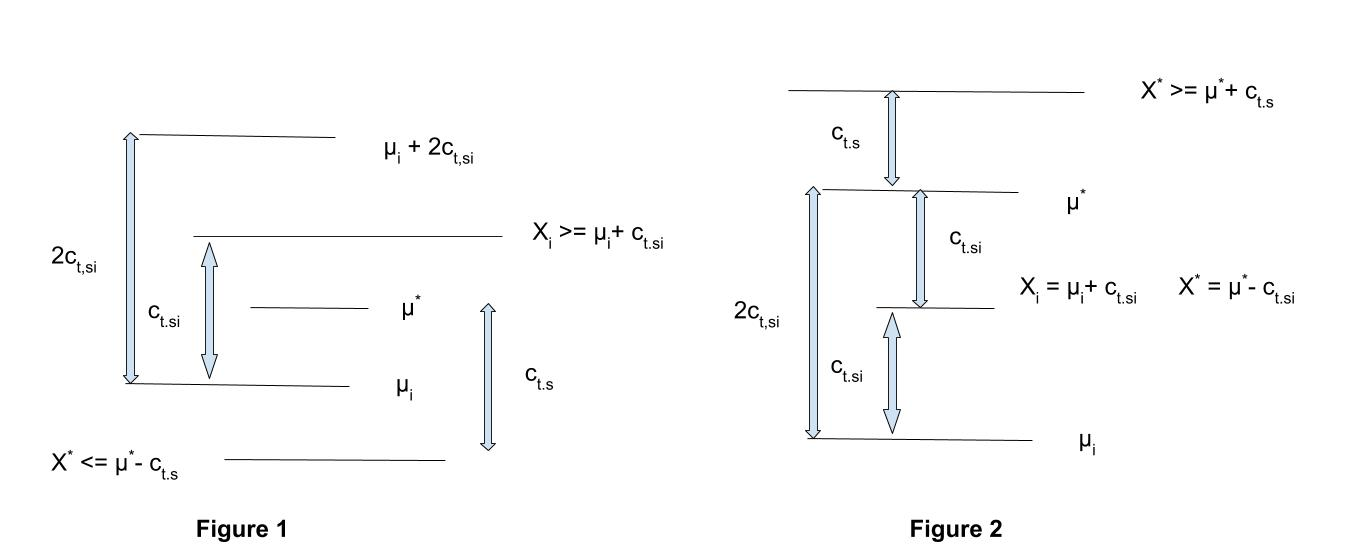
\includegraphics[scale=0.22]{img/UCB1_pic2} 
\item<1-> \begin{align*}
\bar{X}^{*}_{s}\leq \mu^* - c_{t,s};
\bar{X}_{i,s_i}\geq \mu_i + c_{t,s_i};
\mu^*  < \mu_i + 2c_{t,s_i}
\end{align*}
\end{itemize}
\end{frame}

\begin{frame}
\frametitle{UCB1 Proof}
\begin{itemize}
\item<0-> Now, we get the value of confidence interval $c_{t,s_i}=\sqrt{\dfrac{2\ln t}{s_i}}$ by plugging its value in the below equations,
\item<1-> $\mathbb{P}\lbrace  \bar{X}^{*}_{s}\leq \mu^* - c_{t,s}\rbrace\leq \exp\bigg(-2\big(\sqrt{\dfrac{2\ln t}{s}}\big)^2 s\bigg) \leq e^{-4\log t} \leq t^{-4}$
\item<2-> $\mathbb{P}\lbrace \bar{X}_{i,s_i} \geq \mu + c_{t,s_i}\rbrace\leq \exp\bigg(-2\big(\sqrt{\dfrac{2\ln t}{s_i}}\big)^2 s_i\bigg) \leq e^{-4\log t} \leq t^{-4}$
\item<3-> And by plugging $\ell=s_i =\bigg\lceil \dfrac{8\log n}{\Delta_{i}^{2}}\bigg\rceil$ in,
\begin{align*}
\mu^* - \mu_i - 2c_{t,s_i} = \mu^* - \mu_i - 2\sqrt{\dfrac{2\log t}{s_i}} \geq \mu^* - \mu_i -\Delta_i =0
\end{align*} 
we get $\mu^* - \mu_i - 2c_{t,s_i} \geq 0$. So for any pulls greater than $\ell$, $\mu^*$ will surely be atleast $2c_{t,s_i}$  more than $\mu_i$ and one of the rest two events will occur with high probability.
\end{itemize}
\end{frame}

\begin{frame}
\frametitle{UCB1 Proof}
\begin{itemize}
\item<1-> Summing everything up, any sub-optimal arm $i$ will get pulled atleast $\ell$ times and then the two events $\bar{X}^{*}_{s}\leq \mu^* - c_{t,s}$ and $\bar{X}_{i,s_i}\geq \mu + c_{t,s_i}$ will occur with atmost $t^{-4}$ probability.
\item<2-> \begin{align*}
\mathbb{E}[T_{i}(n)]&\leq \bigg\lceil \dfrac{8\log n}{\Delta_{i}^{2}}\bigg\rceil + \sum_{t=1}^{\infty}\sum_{s=1}^{t-1}\sum_{s_i =\ell}^{t-1}2t^{-4}\\
&\leq \dfrac{8\log n}{\Delta_{i}^{2}} +1 + \dfrac{\pi^{2}}{3}, \text{by Bazel's equation}
\end{align*}
\item<3-> So finally the cumulative regret is,
\begin{align*}
\mathbb{E}[R_n]&\leq \sum_{i\in A}\mathbb{E}[T_i (n)]\Delta_i
\leq \sum_{i\in A}\dfrac{8\log n}{\Delta_{i}} + \sum_{i\in A}\Delta_{i}\bigg(1 + \dfrac{\pi^{2}}{3}\bigg)
\end{align*}
\end{itemize}
\end{frame}

\section{PAC Guarantees}
\begin{frame}
\frametitle{Looking beyond Cumulative regret}
\begin{itemize}
\item<1-> Sometimes rather than worrying about cumulative regret we just want to be satisfied with a \emph{nearly good} arm with \emph{high probability}.
\item<2-> This is called the $(\epsilon,\delta)$-guarantee or PAC-guarantee. 
\item<3-> We are interested in finding an arm such that it's $\epsilon$ close to the optimal arm and we can guarantee this with $1-\delta$ probability.
\item<4-> Note, that $\epsilon$ and $\delta$ are given as input and the main aim is to \emph{minimize the number of pulls of an arm $i$ so that it is $\epsilon$ close to the optimal arm with $1-\delta$ probability}. This is called Sample complexity. 
\end{itemize}
\end{frame}

\begin{frame}
\frametitle{A Naive Algorithm}
\begin{algorithm}[H]
\caption{Naive Algorithm}
\begin{algorithmic}[1]
\State Input: $\epsilon > 0$, $\delta > 0$
\State Output: An arm  
\For{each arm $i\in A$}
\State Sample it for $\ell=\dfrac{4}{\epsilon^{2}}\log \dfrac{2K}{\delta}$
\State Let $\bar{X}_i$ be the average reward of arm $i$
\EndFor
\State Output $argmax_{i\in A}\lbrace \bar{X}_i \rbrace$
\end{algorithmic}
\end{algorithm}
\cite{even2006action}
\end{frame}

\begin{frame}
\frametitle{Sample Complexity of Naive Algorithm}
\begin{theorem}
The sample complexity of Naive Algorithm for a set of arms $K$ is given by,
\begin{align*}
O\bigg( \dfrac{K}{\epsilon^2}\log \big( \dfrac{K}{\delta} \big) \bigg)
\end{align*}
\end{theorem}
\cite{even2006action}
\end{frame}

\begin{frame}
\frametitle{Naive Algorithm Sample Complexity Proof}
\begin{itemize}
\item<1-> We want to bound the probability of the event $\bar{X}_i > \bar{X}^* $. The goal is to find the minimum number of pulls required for an arm $i$ so that $\mu^{*}-\mu_i < \epsilon$.
%But by $(\epsilon,\delta)$ definition we need $i$ only to be $\epsilon$ close to $*$.
%Let $\epsilon$ be such that $\mu^* - \mu_i < \epsilon$.
\item<2-> So, we need to bound the opposite condition for sample complexity because till that time we need to pull $i$. Let $i$ be an arm such that $\mu_i<\mu^* - \epsilon \rightarrow \mu_i + \dfrac{\epsilon}{2} <\mu^* - \dfrac{\epsilon}{2}$.
\item<3-> So, we only need to bound the probability of, 
\begin{align*}
\mathbb{P}\lbrace\bar{X}_i > \bar{X}^* \rbrace &\leq \mathbb{P}\bigg\lbrace \bar{X}_i > \mu_i + \dfrac{\epsilon}{2}\bigg\rbrace + \mathbb{P}\bigg\lbrace \bar{X}^* < \mu^* - \dfrac{\epsilon}{2}\bigg\rbrace\\
&\leq 2\exp\bigg(-2\big (\dfrac{\epsilon}{2}\big)^{2}\ell\bigg)\leq 2\exp\bigg(-2\dfrac{\epsilon^2}{4}. \dfrac{4}{\epsilon^{2}}\log \dfrac{2K}{\delta} \bigg)\leq \dfrac{\delta}{K}
\end{align*}
\item<4-> Summing over all the $K-1$ arms (arms excluding $*$) we get, $\dfrac{(K-1)\delta}{K}< \delta$
\end{itemize}
\end{frame}

\begin{frame}
\frametitle{Intuition about Median Elimination}
\begin{itemize}
\item<1-> Can we be more powerful than using Naive Algorithm?
\item<2-> One simple way to modify Naive Algorithm is to divide the time horizon into phases.
\item<3-> In each phase pull all the surviving arms equal number of times.
\item<4-> After that eliminate half the surviving arms with a high guarantee that they are surely not $\epsilon$-optimal arms.
\end{itemize}
\end{frame}

\begin{frame}
\frametitle{Median Elimination}
\begin{algorithm}[H]
\caption{Median Elimination}
\begin{algorithmic}[1]
\State Input: $\epsilon > 0$, $\delta > 0$
\State Output: An arm  
\State Set $S_1 =A$, $\epsilon_1 = \epsilon/4$, $\delta_1=\delta/2$ and $\ell=1$
\For{Repeat till $|S_{\ell}|=1$}
\State Sample every arm in $S_\ell$ for $\dfrac{4}{\epsilon_{\ell}^{2}}\log(\dfrac{3}{\delta_\ell})$ times and let $\bar{X}_i$ denote the average estimated payoff of $i$.
\State Find median $m_{\ell}$ of all surviving arms based on their $\bar{X}_{i},\forall i\in S_\ell$
\State Eliminate all arms from $S_{\ell}$ such that $\bar{X}_{i}< m_{\ell}$ and create $S_{\ell+1}$.
\State Reset Parameters: $\epsilon_{\ell+1}=\dfrac{3}{4}\epsilon$; $\delta_{\ell+1}=\dfrac{1}{2}\delta$; $\ell=\ell+1$
\EndFor
\end{algorithmic}
\end{algorithm}
\cite{even2006action}
\end{frame}

\begin{frame}
\frametitle{Comparison of Median Elimination, Naive Algorithm}

\begin{table}
\caption{Sample Complexity of Median Elimination, Naive Algorithm}
\begin{center}
\begin{tabular}{|c|c|}
\toprule
Algorithm  & Upper bound on Sample Complexity \\
\midrule
Naive        &$O\bigg(\dfrac{K}{\epsilon^2}\log \big( \dfrac{K}{\delta} \big) \bigg)$ \\\midrule
ME      &$O\bigg(\dfrac{K}{\epsilon^2}\log \big( \dfrac{1}{\delta} \big)  \bigg)$\\\bottomrule
\end{tabular}
\end{center}
\end{table}

\begin{itemize}
\item<1-> So clearly Naive algorithm uses more samples than Median Elimination to give us the same $(\epsilon,\delta)$ guarantee
\end{itemize}

\end{frame}




%\begin{frame}
%\frametitle{UCB 1 Experimental Run}
%%\begin{tabbing}
%\begin{center}
%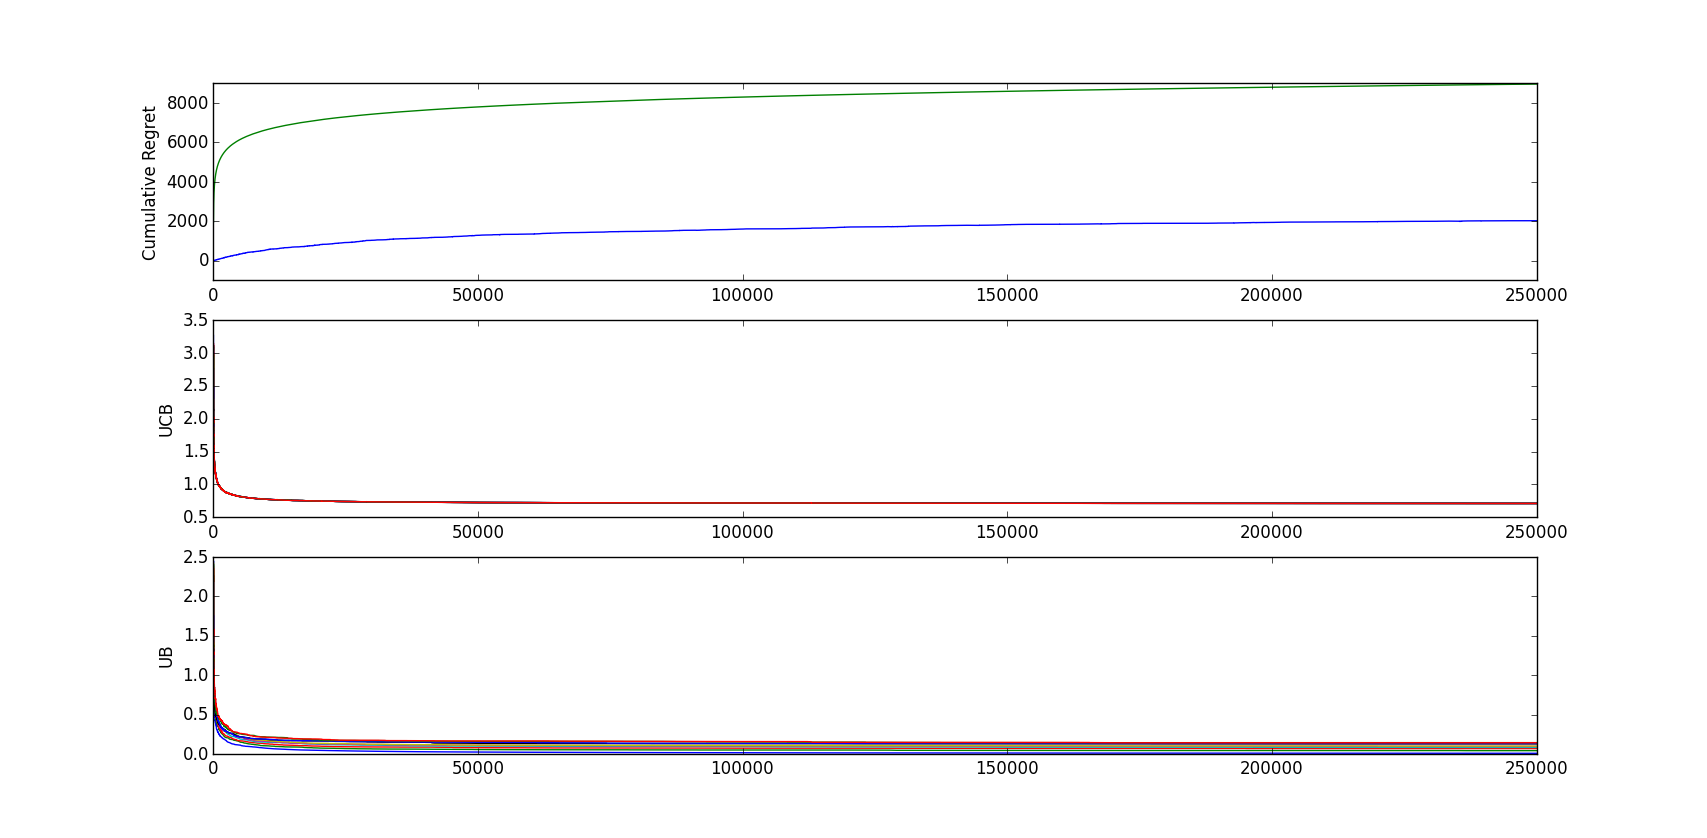
\includegraphics[scale=0.3]{img/ucb.png}
%\end{center}
%\end{frame}

\section{Some Other Bandits} 
\begin{frame}
\frametitle{Some Other Bandits and Applications}

\begin{itemize}
\item Adversarial Bandits : Used in Investment in Stock Markets
\item Contextual Bandits : Used in online Advertisement/news article selection
\item Budgeted Bandits : Used in Clinical trials
\item Distributed Bandits : Used in packet routing through a network
\end{itemize}
\end{frame}

\section{References}
\begin{frame}[allowframebreaks]
\frametitle{References}
\bibliographystyle{plainnat} 
\bibliography{biblio}
\end{frame}


%------------------------------------------------

\begin{frame}
\Huge{\centerline{Thank You}}
\end{frame}

%----------------------------------------------------------------------------------------

\end{document} 